\section{System Architecture} \label{sec:system-architecutre}
\todo[inline]{structure is finalized text is incomplete and not polished}
\todo[inline]{explain the statistics collection unit and the scheduler (in more detail)}
\todo[inline]{update the figure (system architecture)}

The proposed system comprises three main components; model manager, data manager and scheduler, and an independent SGD run-time. 
Figure \ref{fig:system-architecture} gives an overview of the architecture of our system and the interactions among its components.
The data manager first stores the incoming training observations in a buffer and then passes them on to the model manager.
The model manager incrementally updates the model using the training observations.
The model manager is also responsible for receiving prediction requests.
Once it receives a request, it uses the latest version of the model to make a prediction and returns the result to the user.
Both the scheduler and the data manager components are constantly communicating with each other and with the model manager, to obtain the latest statistics, such as the model quality and buffer size.
This in turn helps us to tune the scheduling and sampling rate for future iterations of SGD. 
Next, we explain each component of the system in more detail.


\begin{figure}[t]
\centering
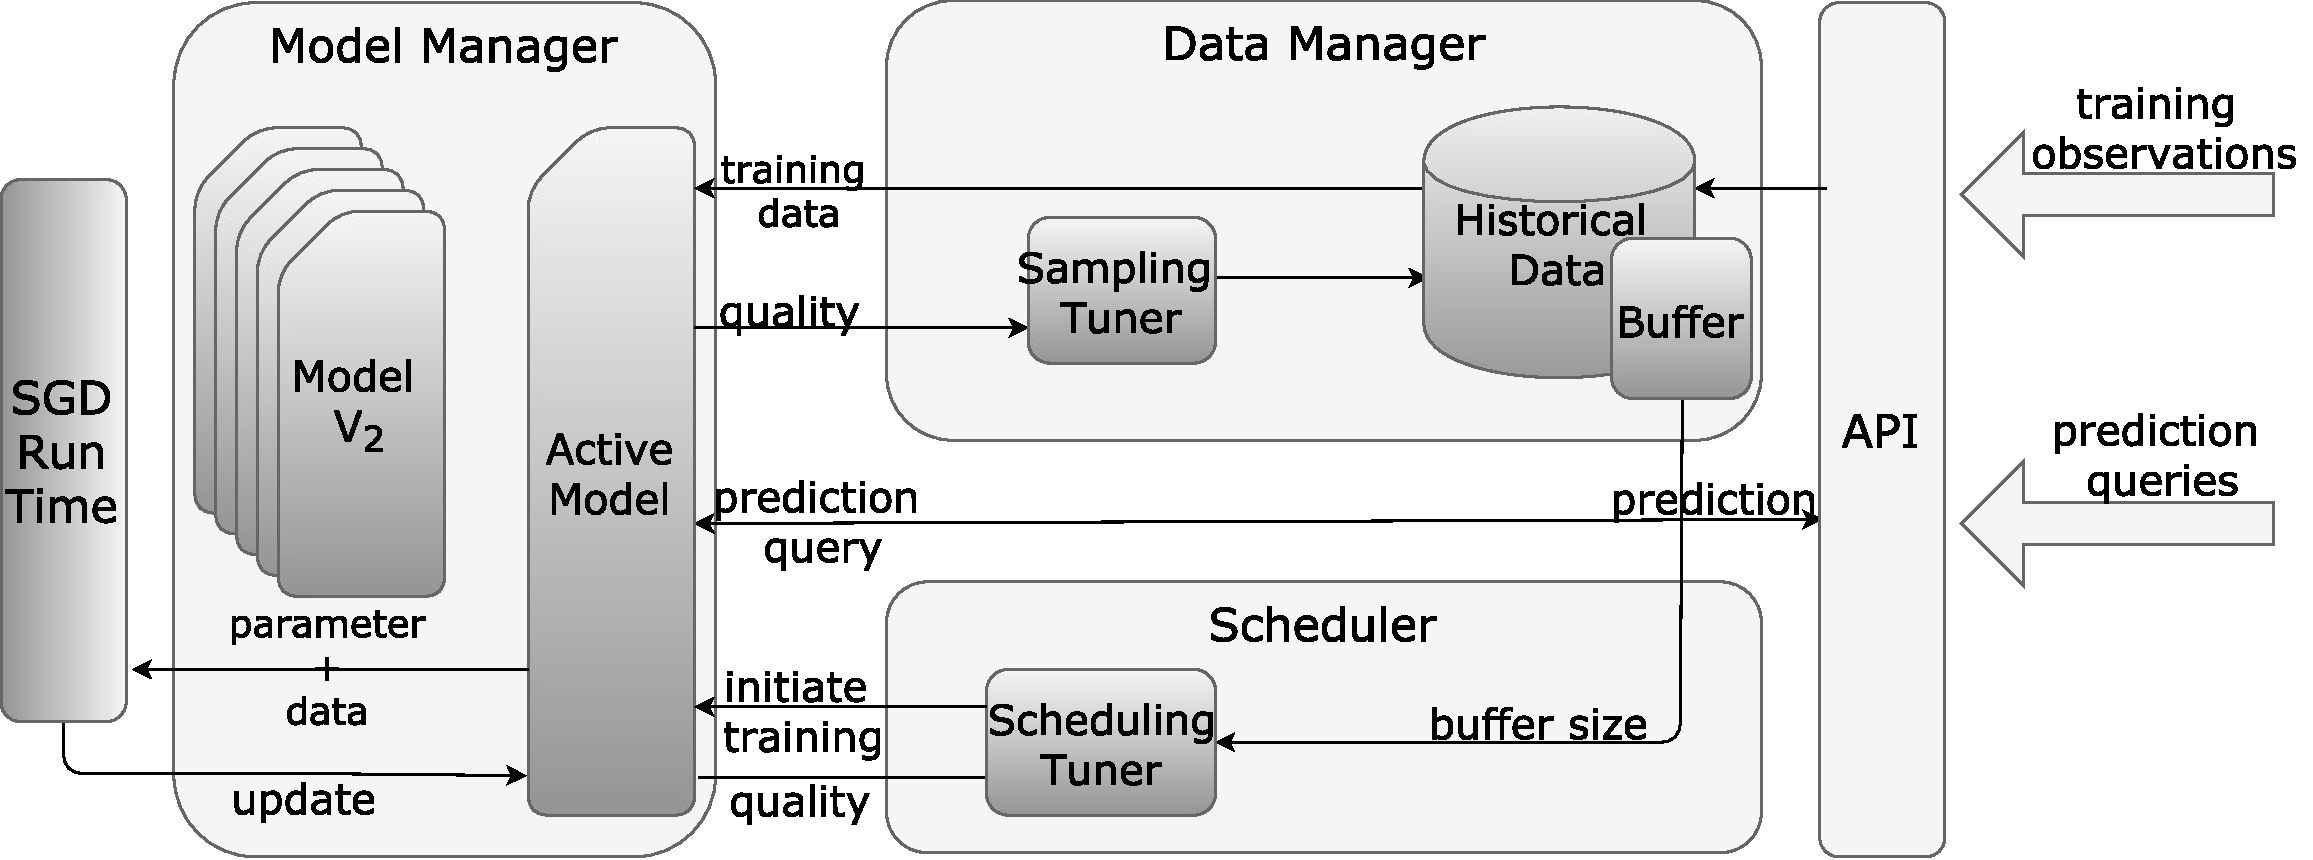
\includegraphics[width=\columnwidth]{../images/system-architecture-final.pdf}
\caption{System Architecture}
\label{fig:system-architecture}
\end{figure}


\subsection{Scheduler}\label{scheduler}
The scheduler component is responsible for scheduling new iterations of SGD.
Intuitively, the best time to execute an iteration is when the system is not under heavy load.
A new iteration of SGD is also executed when the system receives more training data than can be handled by the intermediate buffer.
If the model is not updated with the new training items frequently, the quality decreases.
This decrease in the quality is more rapid if the distribution of the data is changing.
In our prototype, the scheduling rate is controlled by a user defined parameter, \textit{max\_buffer\_size}.
When the intermediate buffer's size reaches \textit{max\_buffer\_size}, the scheduler executes a new iteration of SGD.
It is important to note that the scheduling rate affects the quality of the model.
In Section \ref{evaluation}, we investigate the effect of scheduling rate on model quality.
If no new training data is available, the model parameters will eventually converge and any further training iterations will not have any effect on the model quality.
\todo[inline]{R3: How is the convergence detected?}
Therefore, the scheduler component has to communicate with the model manager in order to detect whether the model parameters have converged and stop further iterations until more training data becomes available.

\subsection{Data Manager} \label{data-manager}
In order to execute an iteration of SGD, we need to combine the training data that arrives at the system in real-time with the data stored on disk.
The data manager is responsible for storing the incoming training observations in an intermediate buffer.
Upon a new training iteration, the data manager accesses the historical data stored on disk and provides a sample.

Different sampling strategies can be used to provide the sample.
In our current prototype, the data manager uses a simple unified random sampling method to generate this sample.
More advanced methods, such as Reservoir \cite{vitter1985random} or weighted random sampling can also be used to generate the sample.
Reservoir sampling is typically used to generate samples from large datasets that do not fit in memory, whereas weighted random sampling is used when data elements have different weights.
In an online machine learning scenario, recent items are more important for training the model and are assigned a bigger weight than older items.
Therefore, weighted random sampling can generate samples that can contribute to the training of a better model.

The data from the sample and the data in the buffer are merged to create the dataset for next training iteration.
The data manager provides access to this dataset for the model manager in order to further train the model.
The data manager also communicates with the scheduler in order to inform it when the intermediate buffer is becoming full and a new training iteration is required. 

The created data set consists of the data inside the buffer and a sample of the historical data as described earlier.
The sampling rate is a system parameter that has to be configured.
It can be pre-configured to a constant value based on the application.
However, using the feedback from the system's model manager (Section \ref{model-manager}), the sampling rate can be adjusted.
For example, when the data distribution is changing, a smaller sampling rate places more emphasis on the data that arrived recently. 
This is similar to the problem of concept drift where the distribution of the incoming data changes overtime.
This renders historical data less important and as a result a smaller sample of the historical data (or none at all) will give more importance to the data in the buffer and help the model to adopt faster to the concept drift.
However, if there is no concept drift in the data, a larger sampling rate will increase the quality of the model after a training iteration.
Another effect that the sampling rate has on the system is the training iteration running time.
A larger sampling rate increases the running time of each training iteration as more data has to be processed.
In Section \ref{evaluation}, we investigate the effects of different sampling rates on both the quality and performance of the system.

Moreover,  new data sets can be registered in data manager.
In our current prototype, new data sets first have to be stored on disk, and data manager can be informed of the data path.
Newly available data sets are used in the subsequent SGD iterations.

\todo[inline]{R2: The difference of incremental update and SGD update needs clarification. In the experiment, they are used in different approaches (baseline+ is using incremental update and Continuous is using SGD). But, the second sentence of the last paragraph of sec 5.3 says both updates are applied in Continuous. BD: I have used incremental to refer to online learning. Whereas in some literature incremental may also refer to mini batch updates. I think the reviewers comment is already addressed in section \ref{subsec:setup}}
\subsection{Pipeline Manager} \label{model-manager} 
\todo[inline]{discuss statistics collection and update the Listing to show apis for statistics gathering. Discuss what are default ones that being collected and how users can have custom statistics collected and use them inside or outside of the system.}
\todo[inline]{Mention how pipelines that are trained outside can be used in the system and how they can be exported again (current prototype uses spark serialized object and we (can) support  PMML}
An important part of the system is the model manager component.
It is responsible for storing the model, answering prediction queries, and performing incremental and batch updates to the model.
Listing \ref{model-manager-api} shows the API of the model manager.
The API is used to interact with other components as well as end-users of the system.
The scheduler component uses \textit{update} and \textit{update\_iteration} to instruct the model manager to perform incremental or batch updates (one iteration of SGD) to the model.
Upon a new prediction query, the \textit{predict} method is called to provide the end-user with the label of the given input.

\noindent\begin{minipage}[t]{\linewidth}
\begin{lstlisting}[language=java, basicstyle=\small\ttfamily, frame=tb ,columns=fullflexible,
showstringspaces=false,label=model-manager-api,caption=Model Manager API, numberstyle=\tiny]
def update(x,y)

def update_iteration(X,Y)

def predict(x): Label

def error_rate(X_test, Y_test): Double

\end{lstlisting}
\end{minipage}


The \textit{error\_rate} method returns the error rate of the model using the provided test dataset.
As described earlier, constant monitoring of the quality is required in order to adjust the scheduling and sampling rate.
When the error rate is stagnating, the model has converged using the existing data.
Therefore the model manager informs scheduler not to schedule any new iterations until new training observations have arrived at the system.
\todo[inline]{R3: How is this done exactly?}
Similarly as explained in Section \ref{data-manager}, an increase in the error rate may indicate a change in distribution of the data.
As a result, reducing the sampling rate will place more emphasis on recent data (in the intermediate buffer) and help adapt the model to the changes in the distribution.

The model manager also keeps track of the changes that are made to the model.
The model is updated both through incremental learning and SGD-iteration.
The model manager creates snapshots of the model in two different scenarios; after a series of incremental updates are made and after each training iteration.
\todo[inline]{R3: What is the algorithm here?}
This versioning of the models is essential.
When there is a rapid change in the distribution of the incoming data (a sudden concept drift) or when there are anomalies in the data, it is sometimes necessary to revert back to a version before the change in distribution occurred.
In case of concept drift, new training iterations should be scheduled that only use the data in the buffer.
Moreover, in case of anomalies in the data, they have to be identified and discarded before any further model updates could happen.

\subsection{SGD Run-Time} 
All components of our model serving system described so far are not limited to any specific run-time.
We have decoupled the components from the actual run time of the system.
Any system capable of performing incremental and batch SGD updates efficiently are suitable options for our system.
Apache Flink \cite{carbone2015apache} and Apache Spark \cite{zaharia2010spark} are distributed data processing platforms that work with data in memory and have support for iterative algorithms, which makes both of them ideal options for our SGD run-time.
In our current prototype, we are using Apache Spark \cite{zaharia2010spark} as our SGD run-time.

The model manager is the component responsible for communicating with the SGD run-time.
In the current version of our prototype, the model manager requests Spark to perform both incremental and batch updates to the model.
Both types of updates are supported by the built in machine learning library of Spark.
The choice of run-time for SGD slightly influences the data manager as well.
In our prototype, historical data is stored on the Hadoop Distributed File System (HDFS) \cite{shvachko2010hadoop}.

\todo[inline]{R3: The paper has a point that not only the resource consumption is reduced by incremental update, but also the prediction accuracy can be improved due to adapting the model to newly seen data. The system uses a sampling component to use a subset of historical data in each SGD update. However, a non-incremental retraining can also achieve the same adaptation by weighing towards the newly seen data (e.g., learning with concept drifting). Therefore, the ideas of incremental update and adaptation to concept drift should not be confused. The evaluation in this paper does not clearly decouple them. BD: Interesting insight. We have to address this.}